\documentclass[UTF8,11pt]{ctexart}

\usepackage[a4paper,margin=2.35cm]{geometry}
\usepackage{amsmath,amssymb,mathtools}
\usepackage{booktabs,array,longtable}
\usepackage{enumitem}
\usepackage{hyperref}
\usepackage{xcolor}
\usepackage[most]{tcolorbox}
\usepackage{tikz}
\usetikzlibrary{arrows.meta,positioning,calc,fit}
\usepackage{listings}

\hypersetup{colorlinks=true,linkcolor=blue!55!black,urlcolor=blue!60!black,citecolor=blue!55!black}
\setlength{\parindent}{2em}
\setlength{\parskip}{0.35em}
\setlist[itemize]{itemsep=0.25em,topsep=0.4em}
\setlist[enumerate]{itemsep=0.25em,topsep=0.4em}

\newcommand{\notetitle}{One Mesh, Many Meanings：一个网格究竟是什么？}
\newcommand{\noteversion}{v0.1}
\newcommand{\notestatus}{teaching}
\newcommand{\notelastupdate}{2026-09-16}
\newcommand{\code}[1]{\texttt{#1}}
\newcommand{\cgalSurfaceMesh}{\texttt{Surface\_mesh}}

\newtcolorbox{keyidea}[1][]{breakable,colback=blue!3,colframe=blue!45!black,title={核心观点 #1},fonttitle=\bfseries}
\newtcolorbox{workedexample}[1][]{breakable,colback=green!3,colframe=green!45!black,title={手算例子 #1},fonttitle=\bfseries}
\newtcolorbox{sidenote}[1][]{breakable,colback=yellow!5,colframe=yellow!45!black,title={支线视野 #1},fonttitle=\bfseries}
\newtcolorbox{failurecase}[1][]{breakable,colback=red!3,colframe=red!50!black,title={失效案例 #1},fonttitle=\bfseries}
\newtcolorbox{exercise}[1][]{breakable,colback=gray!4,colframe=gray!55!black,title={习题 #1},fonttitle=\bfseries}
\newtcolorbox{codingexercise}[1][]{breakable,colback=purple!3,colframe=purple!45!black,title={编码任务 #1},fonttitle=\bfseries}
\newtcolorbox{studentthought}[1][]{breakable,colback=cyan!3,colframe=cyan!45!black,title={Student thought: #1},fonttitle=\bfseries}
\newtcolorbox{assistantresponse}[1][]{breakable,colback=orange!4,colframe=orange!55!black,title={Assistant response (#1)},fonttitle=\bfseries}
\newtcolorbox{versionaddition}[1][]{breakable,colback=violet!3,colframe=violet!50!black,title={Added in #1},fonttitle=\bfseries}

\lstset{basicstyle=\ttfamily\small,columns=fullflexible,frame=single,breaklines=true}

\title{\notetitle}
\author{Mesh 深度学习课程 · M00-N01}
\date{版本 \noteversion\quad 状态：\notestatus\quad 更新：\notelastupdate}

\begin{document}
\maketitle
\tableofcontents

\section*{如何读这篇 Note}
\addcontentsline{toc}{section}{如何读这篇 Note}

这是整门课程的第一篇正式 Note。它故意不从某个经典算法开始，也不从“halfedge 是什么”开始，而先处理一个更基础的问题：

\begin{center}
\Large\bfseries 一个 mesh 到底是哪一种数学对象？
\end{center}

这个问题看似像定义题，实际上会决定后面几乎所有算法的语言。若我们把 mesh 只理解成“很多三角形”，那么拓扑、度量、离散算子、鲁棒性与软件设计会不断混在一起；一旦把层次拆开，很多工程上的怪现象反而会变得非常清楚。

读完本 Note，希望建立五个习惯：

\begin{enumerate}
  \item 看到一个 mesh 时，先问“我现在把它当成 graph、complex、PL surface，还是软件对象？”
  \item 主动区分 \emph{connectivity/topology} 与 \emph{geometry/metric}。
  \item 理解“同一份 $V,F$ 数据”可以承载不同层次的数学意义。
  \item 看到一种数据结构时，不只问怎么存，而问它\textbf{把哪些数学假设写进了表示不变量}。
  \item 遇到算法失败时，先判断坏在组合层、几何层、分析层，还是纯软件层。
\end{enumerate}

\begin{keyidea}
本篇最重要的 taste 是：\textbf{表示从来不是中性的。} 一个数据结构并非只是节省内存的容器；它实际上在声明“我认为输入属于哪一类数学对象，并且我愿意为哪些操作支付常数时间、内存和维护不变量的代价”。
\end{keyidea}

\section{为什么“mesh = 三角形集合”远远不够}

假设有人给我们一个三角网格文件。最直观的理解是：里面有很多点，还有很多三角形。这个理解用于“把东西画出来”常常够用，但一旦开始算法开发，马上会出现一串不同的问题：

\begin{itemize}
  \item 哪些三角形共享一条边？
  \item 一条边能否属于三个面？
  \item 顶点附近是否真的像一个圆盘？
  \item 两个空间坐标完全相同的顶点，是同一个拓扑顶点吗？
  \item 两个三角形穿过彼此，但没有共享边，这个 mesh 还算“合法曲面”吗？
  \item 如果所有坐标不变，只改变三角形连接关系，几何对象发生了什么？
  \item 如果连接关系不变，把顶点移动到另一个位置，拓扑对象发生了什么？
  \item 为什么有的库只要 $V,F$ 两个矩阵，有的库却维护 halfedge、edge、face、handle、property 一大套对象？
\end{itemize}

这些问题之所以显得杂乱，是因为“mesh”这个词实际上同时指向几种不同对象。

\subsection{一条逐层加结构的链}

一种很有用的观察方式是：从最少的信息开始，一层一层给对象增加结构。

\begin{center}
\begin{tikzpicture}[node distance=7mm and 7mm,>=Latex,
  box/.style={draw,rounded corners,align=center,minimum width=3.25cm,minimum height=0.9cm,fill=blue!3}]
  \node[box] (g) {1-skeleton / graph\\顶点与边};
  \node[box,right=of g] (k) {complex\\面与 incidence};
  \node[box,right=of k] (pl) {PL geometry\\坐标、长度、角度};
  \node[box,right=of pl] (a) {analysis\\函数、场、算子};
  \draw[->,thick] (g) -- node[above]{加入面} (k);
  \draw[->,thick] (k) -- node[above]{加入度量/实现} (pl);
  \draw[->,thick] (pl) -- node[above]{加入函数空间} (a);
\end{tikzpicture}
\end{center}

反过来，我们也可以不断“忘掉结构”：

\[
(\text{mesh + fields + operators})
\longrightarrow
(\text{PL geometric mesh})
\longrightarrow
(\text{abstract complex})
\longrightarrow
(\text{graph}).
\]

每忘掉一层，我们会保留某些问题，同时永远失去另外一些问题。

例如：只知道 graph，我们还能问连通性、最短路、度数；但我们已经无法知道一个三角形环到底只是一个圈，还是被一个二维面填满了。

\begin{keyidea}[：忘结构是一种诊断工具]
以后学习算法时，可以不断问：这个算法真正需要哪一层结构？如果一个算法只依赖 connectivity，那么坐标变化不应该改变结果；如果它依赖 metric，那么只保留 graph 就一定不够。这个问题会帮助我们识别算法的本质依赖。
\end{keyidea}

\section{贯穿全篇的四边形例子}

我们先固定一个极小的三角网格，后面所有抽象概念都回到它上面。

取四个顶点
\[
V=\{0,1,2,3\},
\]
坐标为
\[
p_0=(0,0),\quad p_1=(1,0),\quad p_2=(1,1),\quad p_3=(0,1),
\]
以及两个定向三角形
\[
F=\{(0,1,2),(0,2,3)\}.
\]

\begin{center}
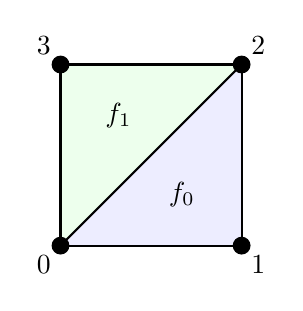
\begin{tikzpicture}[scale=2.3,>=Latex]
  \coordinate (v0) at (0,0);
  \coordinate (v1) at (1,0);
  \coordinate (v2) at (1,1);
  \coordinate (v3) at (0,1);
  \fill[blue!7] (v0)--(v1)--(v2)--cycle;
  \fill[green!7] (v0)--(v2)--(v3)--cycle;
  \draw[thick] (v0)--(v1)--(v2)--(v3)--cycle;
  \draw[thick] (v0)--(v2);
  \foreach \p/\n/\pos in {v0/0/below left,v1/1/below right,v2/2/above right,v3/3/above left}{
    \fill (\p) circle (1.4pt); \node[\pos] at (\p) {$\n$};
  }
  \node at (0.67,0.28) {$f_0$};
  \node at (0.32,0.72) {$f_1$};
\end{tikzpicture}
\end{center}

\subsection{只看 graph 时}

它的边集为
\[
E=\{01,12,02,23,30\}.
\]
此时我们得到一个普通 graph $G=(V,E)$。我们知道 $0$ 与 $2$ 相邻，也知道从 $1$ 到 $3$ 可以经过 $0$ 或 $2$，但 graph 本身并不知道哪三个边围成了一个真正的二维面。

\begin{workedexample}[：一个三角形到底是圈还是面？]
取三个顶点 $\{0,1,2\}$ 与三条边 $\{01,12,20\}$。

若只把它看作 graph，它是一个三边形环，拓扑上相当于圆 $S^1$。

若再声明 $\{0,1,2\}$ 是一个二维 simplex，则这个环被“填满”，整体变成一个三角形盘，拓扑上相当于闭圆盘 $D^2$。

两者拥有完全相同的 1-skeleton，却不是同一个拓扑空间。

因此：\textbf{graph 不是 surface mesh 的全部拓扑信息。}
\end{workedexample}

\subsection{加入二维面：complex 的层次}

对于三角网格，最自然的抽象模型之一是二维 simplicial complex。

\paragraph{定义（抽象 simplicial complex）}
设 $V$ 是顶点集合。一个抽象 simplicial complex $K$ 是 $V$ 的有限非空子集组成的集合，并满足闭包条件：
\[
\sigma\in K,\ \emptyset\neq \tau\subseteq\sigma
\quad\Longrightarrow\quad
\tau\in K.
\]

在二维情形中：
\begin{itemize}
  \item $\{i\}$ 是 0-simplex（顶点）；
  \item $\{i,j\}$ 是 1-simplex（边）；
  \item $\{i,j,k\}$ 是 2-simplex（三角形面）。
\end{itemize}

对于上面的方形例子，两个 2-simplex 自动要求它们的所有边和顶点也属于 $K$。

这里有一个容易被程序员忽略的小点：\textbf{抽象 simplicial complex 中的 simplex 本身是不带方向的集合。} 程序里的 $(0,1,2)$ 顺序还承载了 orientation，这属于额外结构，而不是集合 $\{0,1,2\}$ 本身。

\subsection{加入坐标：geometric realization 与 PL surface}

现在再给每个抽象顶点一个坐标
\[
p:V\to\mathbb R^3.
\]
对于每个 simplex $\sigma=\{i_0,\dots,i_k\}$，我们把它实现成凸包
\[
|\sigma|_p=\operatorname{conv}\{p_{i_0},\dots,p_{i_k}\}.
\]

于是抽象组合对象获得了具体几何形状。

这是第一次真正能够谈：
\[
\text{length},\quad \text{angle},\quad \text{area},\quad \text{normal}.
\]

如果我们保持 $F$ 完全不变，而移动 $p_i$，抽象 complex 没有变化，但几何曲面发生了变化。

\begin{center}
\begin{tikzpicture}[scale=1.7]
  \begin{scope}
    \coordinate (a0) at (0,0); \coordinate (a1) at (1,0);
    \coordinate (a2) at (1,1); \coordinate (a3) at (0,1);
    \draw[thick] (a0)--(a1)--(a2)--(a3)--cycle; \draw[thick] (a0)--(a2);
    \node[below] at (0.5,-0.25) {同一 connectivity：平面实现};
  \end{scope}
  \begin{scope}[xshift=3.0cm]
    \coordinate (b0) at (0,0); \coordinate (b1) at (1.1,0.1);
    \coordinate (b2) at (0.8,1.15); \coordinate (b3) at (-0.15,0.72);
    \draw[thick] (b0)--(b1)--(b2)--(b3)--cycle; \draw[thick] (b0)--(b2);
    \node[below] at (0.45,-0.25) {同一 connectivity：另一实现};
  \end{scope}
\end{tikzpicture}
\end{center}

\begin{sidenote}[：intrinsic geometry 不一定需要三维坐标]
对一个三角 complex，我们甚至可以不先给 $p_i\in\mathbb R^3$，而只给每条边一个长度 $\ell_{ij}>0$，要求每个三角形满足三角不等式。于是每个面本身都可以被看成一个欧氏三角形，再沿公共边粘起来。

这给出了一个 piecewise-Euclidean intrinsic metric。它未必对应你当前看到的某个三维嵌入，但测地距离、角度亏损等内蕴几何量已经可以定义。

这个观点以后会直接通向 intrinsic triangulation、离散曲率与 Delaunay 的内蕴版本。
\end{sidenote}

\subsection{再加入函数：分析对象出现}

假设在每个顶点上存一个温度
\[
u:V\to\mathbb R.
\]
现在 mesh 不只是“曲面”，还是一个承载离散函数的计算域。

以后我们会逐步构造
\[
\nabla_h u,\qquad \operatorname{div}_h X,\qquad \Delta_h u,
\]
讨论 Poisson 方程、heat equation、谱分解等。

注意：这些算子并不是凭空从 $V,F$ 两个数组里长出来的。它们通常同时需要：

\begin{itemize}
  \item incidence/topology：谁和谁相邻；
  \item metric/geometry：长度、面积、角度；
  \item function space：未知量放在顶点、边、面，还是更一般的 cochain 上。
\end{itemize}

这就是后面 M04 中 FEM、DEC、cotangent Laplacian 会汇合的地方。

\section{orientation：一个微小的顺序，如何变成全局结构}

回到两个面
\[
f_0=(0,1,2),\qquad f_1=(0,2,3).
\]
它们都按逆时针方向排列。内部公共边 $02$ 在第一个面边界中以 $2\to0$ 出现，在第二个面中以 $0\to2$ 出现；方向恰好相反。

这件事并非排版习惯，而是曲面 orientation 的离散影子。

\begin{workedexample}[：边界算子让内部边自动消失]
把一个定向三角形记作 $[i,j,k]$。链复形中的边界算子为
\[
\partial[i,j,k]=[j,k]-[i,k]+[i,j].
\]
于是
\[
\partial[0,1,2]=[1,2]-[0,2]+[0,1],
\]
\[
\partial[0,2,3]=[2,3]-[0,3]+[0,2].
\]
两式相加：
\[
\partial\bigl([0,1,2]+[0,2,3]\bigr)
=[0,1]+[1,2]+[2,3]-[0,3].
\]
内部对角线 $[0,2]$ 完全抵消，只剩真正的外边界。

这里已经提前出现了后续拓扑课程的核心结构：\textbf{内部 incidence 通过符号成对抵消，边界是无法抵消的部分。}
\end{workedexample}

这也是一个很好的例子：程序中的 face winding、数学上的 orientation、线性代数里的 incidence matrix，其实是同一结构的不同语言。

\section{局部结构：star、link 与“像不像一个曲面”}

“每个面都是三角形”仍然不足以保证整体是二维流形。

一个真正的二维流形，在每个内部点附近应该局部像一个二维圆盘；在边界点附近则像半圆盘。

在 simplicial complex 中，这种局部结构可以通过 \emph{link} 看到。

\subsection{直觉定义}

对顶点 $v$：

\begin{itemize}
  \item $\operatorname{star}(v)$：所有包含 $v$ 的 simplex，以及它们的面；
  \item $\operatorname{link}(v)$：把这些 simplex 里的 $v$ 去掉之后，围绕 $v$ 留下来的“边界形状”。
\end{itemize}

对于一个良好的三角曲面：

\[
\operatorname{link}(v)\cong
\begin{cases}
S^1, & v\text{ 是内部顶点},\\
[0,1], & v\text{ 是边界顶点}.
\end{cases}
\]

\begin{center}
\begin{tikzpicture}[scale=1.4]
  \begin{scope}
    \coordinate (c) at (0,0);
    \foreach \ang/\n in {45/0,135/1,225/2,315/3}{\coordinate (p\n) at (\ang:1);}
    \draw[thick] (p0)--(p1)--(p2)--(p3)--cycle;
    \foreach \n in {0,1,2,3}{\draw[thick] (c)--(p\n);}
    \fill (c) circle (1.5pt); \node at (0,-0.23) {$v$};
    \node[below] at (0,-1.25) {内部顶点：link 是一个圈};
  \end{scope}
  \begin{scope}[xshift=4.0cm]
    \coordinate (b) at (0,0);
    \coordinate (q0) at (-1,0); \coordinate (q1) at (-0.4,0.9);
    \coordinate (q2) at (0.4,0.9); \coordinate (q3) at (1,0);
    \draw[thick] (q0)--(q1)--(q2)--(q3);
    \foreach \q in {q0,q1,q2,q3}{\draw[thick] (b)--(\q);}
    \fill (b) circle (1.5pt); \node[below] at (b) {$v$};
    \node[below] at (0,-1.25) {边界顶点：link 是一条链};
  \end{scope}
\end{tikzpicture}
\end{center}

\begin{failurecase}[：三个三角形共用同一条边]
如果一条边同时属于三个面，那么这条边附近不再像一个平面条带。组合上，这已经不是通常意义下的 2-manifold edge。

很多标准 halfedge 结构把一条无向边建模成恰好两个相反方向的 halfedges；“第三个面”不是一个普通 corner case，而是在破坏数据结构背后的数学对象假设。

因此看到库报错时，正确的问题不是立刻问“怎么绕过这个检查”，而是先问：\textbf{这个库声称表示的是一般 cell complex，还是 oriented manifold surface？}
\end{failurecase}

完整的 manifold、orientability、boundary 与 homology 会在 M01 展开。本节只希望留下一个印象：\textbf{局部 topology 是算法前置条件的一部分，而不是网格清洗时才处理的脏数据。}

\section{软件里的 mesh：表示的是对象，还是操作？}

数学家可以写一句“令 $K$ 是一个有限二维 simplicial complex”，然后开始证明。

程序却必须回答：

\begin{itemize}
  \item 给定顶点，如何快速枚举相邻面？
  \item edge collapse 后，哪些索引失效？
  \item 属性存在顶点还是面？拓扑修改后它们怎么更新？
  \item 是否允许 non-manifold edge？
  \item 删除元素后是否保持 handle 稳定？
  \item 数据要不要连续存储，是否适合 SIMD / GPU / sparse assembly？
\end{itemize}

因此，软件数据结构可以理解为：

\[
\boxed{\text{Mathematical object} + \text{representation invariants} + \text{operation priorities}}
\]

\subsection{Indexed Face Set：$V,F$ 为什么如此强大}

最常见的三角网格表示之一是
\[
V\in\mathbb R^{n\times 3},\qquad
F\in\mathbb N^{m\times 3}.
\]

$V$ 第 $i$ 行是顶点坐标，$F$ 第 $j$ 行是第 $j$ 个三角形的三个顶点索引。

libigl 明确采用这一风格，并强调它与 Eigen 矩阵计算自然结合。官方教程中，三角 mesh 就以 \code{MatrixXd V} 和 \code{MatrixXi F} 表示。

它的优点非常直接：

\begin{itemize}
  \item 内存布局简单，通常 cache-friendly；
  \item I/O、复制、序列化容易；
  \item 与线性代数、稀疏矩阵、GPU buffer 很自然；
  \item 很多只读 geometry-processing 算法可以写成接近数学公式的矩阵操作。
\end{itemize}

但它没有显式保存“某条边左右各是谁”“围绕一个顶点的面按什么顺序”等局部 adjacency。需要时通常先扫描 $F$ 构造辅助结构。

\begin{keyidea}[：$V,F$ 不是低级，halfedge 也不是高级]
它们优化的是不同操作。

如果算法主要是静态线性代数：$V,F$ 往往极其干净。

如果算法不断做 edge split/collapse/flip，并频繁遍历 one-ring：显式 connectivity 往往值得付出额外存储和不变量维护成本。

选择数据结构前，先问 workload，而不是问哪个“更专业”。
\end{keyidea}

\subsection{Halfedge：把局部 incidence 变成一等公民}

halfedge 的核心动作非常简单：把每条无向边拆成带方向的半边。

对于一个典型的 oriented manifold halfedge representation，每个 halfedge $h$ 会关联若干基本映射：

\[
\operatorname{next}(h),\qquad
\operatorname{twin}(h),\qquad
\operatorname{vertex}(h),\qquad
\operatorname{face}(h).
\]

\begin{center}
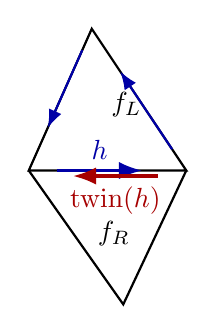
\begin{tikzpicture}[scale=2.0,>=Latex]
  \coordinate (a) at (0,0); \coordinate (b) at (1,0);
  \coordinate (c) at (0.4,0.9); \coordinate (d) at (0.6,-0.85);
  \draw[thick] (a)--(b)--(c)--cycle;
  \draw[thick] (a)--(d)--(b);
  \draw[->,very thick,blue!65!black] ($(a)!0.18!(b)$) -- ($(a)!0.72!(b)$) node[midway,above] {$h$};
  \draw[->,very thick,red!65!black] ($(b)!0.18!(a)+(0,-0.035)$) -- ($(b)!0.72!(a)+(0,-0.035)$) node[midway,below] {$\operatorname{twin}(h)$};
  \draw[->,thick,blue!65!black] ($(b)!0.15!(c)$)--($(b)!0.70!(c)$);
  \draw[->,thick,blue!65!black] ($(c)!0.15!(a)$)--($(c)!0.70!(a)$);
  \node at (0.62,0.42) {$f_L$}; \node at (0.54,-0.40) {$f_R$};
\end{tikzpicture}
\end{center}

\code{next} 让我们沿一个面循环，\code{twin} 让我们跨过一条边。不同库会选择略有不同的 convention：halfedge 指向 head 还是从 tail 出发，边界是否使用 exterior halfedge，删除后如何处理 index 等，但思想相同：\textbf{把 incidence relation 编码成局部常数时间导航。}

\begin{sidenote}[：halfedge 甚至可以被看成 permutation]
geometry-central 的实现文档给出了一个很漂亮的观点：在其 manifold halfedge 表示里，可以通过索引安排让 \code{twin} 近乎隐式，而用一个 permutation array 编码 \code{next}；face 可以看作 \code{next} 的轨道，edge 可以看作 \code{twin} 的轨道。

这正是“代数结构自然融入工程”的一个微型例子：一个看似指针繁多的数据结构，底层其实可以被压缩成若干置换与索引数组。
\end{sidenote}

\subsection{边界为什么总让实现细节变多}

内部 edge 很舒服：两侧各一个 face。

边界 edge 只有一侧有真实面。库可以有不同策略：

\begin{itemize}
  \item \code{twin} 指向一个特殊 invalid/null face；
  \item 显式创建 exterior halfedge，并把整条 boundary loop 当作某种虚拟 face；
  \item 在 general surface mesh 中放宽“恰好一个 twin”的假设，改成 sibling orbit。
\end{itemize}

这些不是数学上谁对谁错，而是不同 representation contract。

例如 geometry-central 的 \code{ManifoldSurfaceMesh} 使用 exterior halfedges 来让 boundary traversal 保持统一，而其更一般的 \code{SurfaceMesh} 可以用 sibling 关系处理一条 edge 上多个 halfedges 的情况。

\subsection{四个成熟库，四种 taste}

下面不是排名，只是观察“同一个 mesh 概念如何被不同设计哲学编码”。

\begin{center}
\small
\begin{tabular}{p{2.2cm}p{3.4cm}p{4.0cm}p{4.2cm}}
\toprule
库 & 主要对象风格 & 擅长表达的 workload & 值得观察的设计点\\
\midrule
libigl & $V,F$ 矩阵 + 函数 & 静态 geometry processing、线性代数、快速研究原型 & 极少状态；connectivity 常按需构造；数学公式与 Eigen 表达接近\\
\addlinespace
OpenMesh & halfedge + typed handles + iterators/circulators + properties & 动态 polygon mesh、邻域遍历、局部拓扑操作 & trait/property 系统；handle 抽象；经典 halfedge API\\
\addlinespace
geometry-central & index-based surface mesh + 独立 geometry hierarchy & DDG、intrinsic/extrinsic geometry、动态 mesh & connectivity 与 geometry 明确分层；dense buffer；general 与 manifold mesh 分开\\
\addlinespace
CGAL \cgalSurfaceMesh & index-based halfedge + runtime property maps + graph concepts & 作为 CGAL 各类 polygon mesh algorithm 的通用载体 & descriptor/type safety；BGL 概念兼容；删除/garbage collection；运行时 property\\
\bottomrule
\end{tabular}
\end{center}

这里最值得训练的能力不是背 API，而是读源码时问：

\begin{enumerate}
  \item 它把什么当作一等对象？vertex、halfedge、corner、face，还是纯矩阵？
  \item 哪些关系显式存储，哪些按需推导？
  \item 哪些不变量是构造时检查的，哪些由调用者负责？
  \item mutation 后 handle/property 如何保持一致？
  \item geometry 是否与 connectivity 解耦？
\end{enumerate}

\section{同一个“坏网格”，可能坏在完全不同的层}

这是本篇最重要的工程诊断部分。

\begin{center}
\small
\begin{longtable}{p{3.0cm}p{3.4cm}p{4.2cm}p{4.2cm}}
\toprule
现象 & 首先坏在哪一层 & 数学解释 & 典型工程后果\\
\midrule
索引越界 & 软件表示层 & 根本无法解释成预期 combinatorial object & crash、UB、错误访问\\
\addlinespace
一个 face 重复使用同一顶点，如 $(0,0,1)$ & complex / geometry 边界处 & 不是正常 2-simplex；几何面积也退化为零 & normal/area/局部算子异常\\
\addlinespace
三个 face 共一条 edge & 组合拓扑层 & edge neighborhood 非 2-manifold & 标准 twin 假设失败；collapse/parameterization 等算法前提失效\\
\addlinespace
相邻 face winding 不一致 & orientation 层 & 共享边不能以相反诱导方向一致抵消 & normal 翻转、inside/outside 混乱、边界提取错误\\
\addlinespace
两个不同 vertex index 坐标完全相同 & topology 与 geometry 不一致 & 几何上重合，不代表组合上粘合 & 看起来闭合但拓扑有裂缝；welding 前后 topology 改变\\
\addlinespace
远处两个 triangle 在空间中互相穿过 & geometric realization 层 & 抽象 complex 仍可能是流形，但映射到 $\mathbb R^3$ 不是 embedding & Boolean、inside/outside、collision、制造流程出问题\\
\addlinespace
极瘦但非退化 triangle & metric / numerical layer & topology 完全合法，但 metric quality 很差 & FEM conditioning、normal/curvature estimate、remeshing 质量恶化\\
\addlinespace
删除元素后旧 handle 仍被使用 & 软件生命周期层 & 数学对象未必有问题，identity mapping 已失效 & 隐蔽逻辑 bug\\
\bottomrule
\end{longtable}
\end{center}

\begin{failurecase}[：坐标重合不等于拓扑粘合]
假设两个三角形在文件里各自有一个顶点，两个顶点坐标都是 $(0,0,0)$，但索引分别是 17 和 203。

渲染时它们可能看起来无缝接触；在 abstract complex 中，它们却仍是两个完全不同的 0-simplex。

如果你做一次 vertex welding，把二者合并为同一 index，你执行的不是“数值清洗”这么简单，而是\textbf{改变了组合拓扑}。

因此任何 weld tolerance 都隐含一个建模假设：多近才应该被视为同一个拓扑实体？这已经不是纯数据结构问题。
\end{failurecase}

\begin{failurecase}[：组合流形不保证空间中没有自交]
可以构造一个 abstract triangulated disk，使每个 edge incidence、vertex link 都完全满足 manifold 条件，然后把坐标移动到两个远处三角形互相穿过的位置。

此时 combinatorial topology 没坏，local manifold test 也可能全过；坏的是实现到 $\mathbb R^3$ 的几何 embedding。

这就是为什么“manifold mesh”和“self-intersection-free embedded surface”是两个不同条件。
\end{failurecase}

\section{一个极小但重要的工程任务：MeshAudit}

第一篇 Note 就应该产生一点可复用代码，但不急着造完整 halfedge kernel。

我建议 Mesh Algorithm Library 的第一个真实组件不是 \code{HalfedgeMesh}，而是一个针对 indexed triangle mesh 的 \textbf{MeshAudit / validation layer}。

理由很简单：如果我们还没有清楚区分合法性层次，就过早设计复杂数据结构，很容易把若干假设偷偷写死。

\begin{codingexercise}[：实现第一版 MeshAudit]
输入：
\[
V\in\mathbb R^{n\times 3},\qquad F\in\mathbb Z^{m\times 3}.
\]

第一版至少输出以下诊断：

\begin{enumerate}
  \item \textbf{storage validity}：所有索引是否在 $[0,n)$；
  \item \textbf{face validity}：一个 face 是否包含重复 index；
  \item \textbf{edge incidence}：建立无向边表，统计每条边 incident face 数；
  \item \textbf{boundary classification}：incident count 为 1 的边；
  \item \textbf{non-manifold edge}：incident count $>2$；
  \item \textbf{orientation consistency}：两个相邻三角形是否在共享边上诱导相反方向；
  \item \textbf{Euler data}：$|V|,|E|,|F|,\chi=|V|-|E|+|F|$；
  \item \textbf{geometric degeneracy}：面积为零或接近零的 triangle；
  \item \textbf{duplicate-position report}：坐标相同/极近但 index 不同的 vertex，只报告，不自动 weld。
\end{enumerate}

暂时\textbf{不要求}完整解决 vertex-nonmanifold、self-intersection、orientability of arbitrary components、robust tolerance policy；这些会随着 M01/M11/M03 的理论推进逐步升级。

设计要求：诊断结果必须注明属于哪一层，例如
\begin{lstlisting}
[TOPOLOGY] edge (10, 31) has 3 incident faces
[ORIENTATION] faces 7 and 18 use edge (4, 9) in same direction
[GEOMETRY] face 51 has near-zero area
[REPRESENTATION] face 3 references vertex 1024 >= nVertices
\end{lstlisting}

这比单一 \code{isValid(mesh)} 更有教学价值，也更有工程价值。
\end{codingexercise}

\section{为什么成熟库值得读：不是为了复制，而是为了观察取舍}

本课程后面会反复阅读成熟库，但目的不是把它们当“标准答案”。

例如：

\begin{itemize}
  \item libigl 让我们观察：当绝大多数任务是静态数值算法时，重型 mesh object 是否真的必要？
  \item OpenMesh 让我们观察：一个通用 halfedge 库如何组织 handle、circulator、property 与 mutation；
  \item geometry-central 让我们观察：connectivity、intrinsic geometry、extrinsic geometry 能否被明确分层；
  \item CGAL 让我们观察：当 mesh 需要进入庞大 generic algorithm ecosystem 时，graph concepts、descriptors、property maps 如何成为接口语言。
\end{itemize}

我们最终自己的库不应该一开始试图综合所有优点。相反，课程会先积累真实算法需求，再决定抽象。

\begin{keyidea}[：接口应由算法压力长出来]
课程长期目标是 Mesh Algorithm Library，但第一原则仍然是：\textbf{不要为了未来统一而过早抽象。}

每一次新增数据结构，都应该能够回答：是哪一类算法反复需要它？它消除了什么复杂度？它引入了哪些新的不变量与维护成本？
\end{keyidea}

\section{视野：同样叫 mesh，不同领域其实在离散不同东西}

“mesh 被广泛使用”并不是因为三角形特别神奇，而是因为它提供了一种把连续对象变成有限可计算对象的方法。

\subsection{图形学：离散的是可见表面}

渲染里，surface mesh 主要近似物体边界。很多时候最重要的是：位置、法向、UV、材质属性，以及 GPU 友好的三角 primitive。

\subsection{CAD tessellation：离散的是精确参数曲面}

B-Rep/NURBS 中的曲面本身可能有精确参数表达；mesh 是为了显示、碰撞、下游交换或近似计算生成的离散代理。

此时误差问题自然出现：弦差、法向误差、参数域采样、trim boundary 等。

\subsection{有限元：离散的是计算域与函数空间}

FEM 中 mesh 不只是“画一个形状”，而是定义 basis function 支撑、数值积分单元、自由度邻接与离散 PDE 的骨架。

于是 element quality 会影响 conditioning 与 approximation，而不只是视觉三角形好不好看。

\subsection{视觉/扫描：mesh 可能是逆问题的输出}

点云、深度图甚至图像先给出不完整观测，mesh 是对隐藏连续表面的一个假设与重建结果。

这会在 M12 把我们带向 point set、implicit surface，再进一步连接 neural/explicit scene representation。

\begin{sidenote}[：这也是为什么未来不应执着于“mesh 才是几何”]
mesh 是极其成功的一类有限表示，但它不是几何世界的终点。point cloud、voxel、level set、SDF、B-Rep、subdivision surface、NeRF、Gaussian representation 都是在为不同任务选择不同的“可计算对象”。

真正值得掌握的能力不是忠于某一种表示，而是判断：\textbf{当前任务要求保存什么结构，允许牺牲什么结构？}
\end{sidenote}

\section{习题：不是检查记忆，而是建立对象层次感}

\begin{exercise}[1：把方形例子完整拆成四层]
对本文的两三角形方形：

\begin{enumerate}
  \item 写出 graph $G=(V,E)$；
  \item 写出完整 simplicial complex $K$ 中所有 0-, 1-, 2-simplices；
  \item 写出两个面的定向边界，并验证内部边抵消；
  \item 把 $p_2$ 改成 $(1,1,1)$（嵌入 $\mathbb R^3$），说明哪些结论改变、哪些完全不变；
  \item 再把 $p_2$ 改成 $p_0$，判断 topology、abstract complex、geometric realization 分别发生了什么。
\end{enumerate}
\end{exercise}

\begin{exercise}[2：相同 1-skeleton，不同空间]
给定三角形 graph $C_3$。比较：
\[
K_1=\{\text{三个顶点与三条边}\},
\qquad
K_2=K_1\cup\{\{0,1,2\}\}.
\]

不要只说“一个有面一个没面”。请从以下角度比较：
\begin{itemize}
  \item 哪些 loop 可以被填掉？
  \item Euler characteristic 有何不同？
  \item 如果只保存 adjacency matrix，能否区分二者？
\end{itemize}

这是后续 chain/homology 语言的预热。
\end{exercise}

\begin{exercise}[3：representation contract]
假设你要实现下面三个算法：

\begin{enumerate}
  \item 对固定三角网格组装 cotangent Laplacian；
  \item 连续执行十万次 edge flip；
  \item 把一百万三角形流式上传到 GPU 渲染。
\end{enumerate}

分别讨论 $V,F$、halfedge、corner-table/专用压缩表示各自的优劣。不要回答“哪个最快”，而要明确列出：
\[
\text{需要的 primitive query} + \text{mutation pattern} + \text{memory pattern}.
\]
\end{exercise}

\begin{exercise}[4：构造一个“拓扑合法但几何非法”的例子]
手画或用代码构造一个三角 mesh：

\begin{itemize}
  \item 每条 interior edge 恰好两个 incident faces；
  \item 每个 vertex 的 link 满足流形条件；
  \item 但两个不相邻的三角形在 $\mathbb R^3$ 中发生自交。
\end{itemize}

然后解释为什么一个只检查 adjacency 的 validator 无法发现问题。
\end{exercise}

\begin{exercise}[5：读库，不写代码]
任选 libigl、OpenMesh、geometry-central、CGAL \cgalSurfaceMesh 中两个，回答：

\begin{enumerate}
  \item mesh element 的 identity 如何表示？
  \item adjacency 是显式还是隐式/按需？
  \item geometry 是否与 topology 分离？
  \item 删除 element 后 identity 怎么处理？
  \item 如果输入有 non-manifold edge，它选择拒绝、特殊表示还是放宽结构？
\end{enumerate}

这道题的目标不是 API 熟练，而是训练“从代码设计反推数学假设”。
\end{exercise}

\section{本篇的最低掌握标准}

在进入下一篇之前，不要求背任何库 API，但希望能够自然地说清楚下面几句话：

\begin{enumerate}
  \item 一个 surface mesh 可以被看成 graph，但 graph 会忘掉 face incidence。
  \item abstract simplicial complex 描述组合粘合；orientation 是额外结构。
  \item vertex coordinates / edge lengths 给组合对象加入几何；同一 topology 可以有许多 realization。
  \item combinatorial manifold、embedded non-self-intersecting surface、high-quality numerical mesh 是三个不同条件。
  \item $V,F$ 与 halfedge 没有谁“更正确”；它们在为不同 primitive operations 付费。
  \item 一个成熟 mesh library 的数据结构设计，本质上是一组关于对象类别、允许操作与不变量的承诺。
\end{enumerate}

如果这六句话已经成为直觉，M00 的第一步就完成了。

\section{下一步预告}

M00 后续 Note 暂定继续处理两件事：

\begin{enumerate}
  \item 从 polygon soup 到可导航 surface mesh：incidence、boundary、orientation 与 halfedge 的更细实现；
  \item 真实成熟库解剖：选择两到三个库，把同一个极小 mesh 的构造、遍历、属性与修改逐项对照。
\end{enumerate}

但是否按这个顺序继续，要根据你阅读本 Note 后的批注决定。若你认为数学对象层次仍不够深，M01 的部分内容可能提前；若你认为工程感觉不足，也可以先做一个短的 library lab。

\section*{References}
\addcontentsline{toc}{section}{References}

\subsection*{本篇直接推荐}

\begin{enumerate}
  \item Mario Botsch, Leif Kobbelt, Mark Pauly, Pierre Alliez, Bruno L\'evy, \emph{Polygon Mesh Processing}. 作为传统 geometry processing 的主参考之一，尤其关注 mesh representation/data structure 与经典 surface-processing 语境。

  \item Keenan Crane 等，\emph{Discrete Differential Geometry: An Applied Introduction}. 本篇只需要它关于离散曲面/三角网格的整体视角；后续 M02--M06 会更重要。

  \item Lutz Kettner, ``Using Generic Programming for Designing a Data Structure for Polyhedral Surfaces,'' \emph{Computational Geometry}, 13(1), 1999, 65--90. 很适合从“数学 combinatorial structure 如何变成通用 C++ library design”这一角度精读。
\end{enumerate}

\subsection*{工程文档（建议边读边看源码）}

\begin{itemize}
  \item libigl tutorial: \url{https://libigl.github.io/tutorial/}
  \item geometry-central surface mesh basics/internals: \url{https://geometry-central.net/surface/surface_mesh/basics/} ，\url{https://geometry-central.net/surface/surface_mesh/internals/}
  \item geometry-central geometry hierarchy: \url{https://geometry-central.net/surface/geometry/geometry/}
  \item CGAL \cgalSurfaceMesh{} manual: \url{https://doc.cgal.org/latest/Surface_mesh/index.html}
  \item OpenMesh documentation: \url{https://www.graphics.rwth-aachen.de/media/openmesh_static/Documentations/OpenMesh-8.1-Documentation/index.html}
\end{itemize}

\subsection*{Requested References：希望你补充到项目里的资料}

下面不是开课硬阻塞，但如果方便，希望优先补进项目文件库或仓库可访问资料中。后续 Note 会直接精读，而不是只依赖二手介绍。

\begin{enumerate}
  \item \textbf{高优先级：}Botsch et al., \emph{Polygon Mesh Processing} 完整版本。第一阶段主要用于 M00 的数据结构、M07--M11 的经典算法对照。

  \item \textbf{高优先级：}Lutz Kettner, \emph{Using Generic Programming for Designing a Data Structure for Polyhedral Surfaces} (1999) 完整论文。虽然网上可找到版本，但若项目中有固定 PDF，后续做源码/设计思想对照会更稳定。

  \item \textbf{中优先级：}你手头若已有 OpenMesh / CGAL / geometry-central 相关的论文、设计文档或课程材料，可以补充。我们真正想看的不是 API 文档，而是作者为何选择这些抽象。

  \item \textbf{中优先级：}Keenan Crane 的 DDG 讲义当前完整版本。公开版本通常可以直接获取，但如果你希望课程长期固定在某一版上，建议上传一份作为项目基准。
\end{enumerate}

如果后续你找到其他经典 mesh data structure 论文（例如 directed-edge、corner table、quad-edge 等），也可以先放入 refs；我会在需要时决定是否升级成 side-note，而不是现在全部塞进主线。

\section*{Revision history}
\addcontentsline{toc}{section}{Revision history}

\begin{itemize}
  \item \textbf{v0.1 — 2026-09-16}: Initial teaching draft. 建立 mesh 的 graph / complex / PL geometry / analysis / software-object 五层视角；加入方形手算、orientation 边界抵消、star/link 预览、$V,F$ 与 halfedge 对照、成熟库设计观察、分层失效诊断、MeshAudit 编码任务与首批习题。
\end{itemize}

\end{document}